\documentclass[11pt, letterpaper]{beamer}

% title and declarations
\title{The Tile Game}
\subtitle{lol why did i make this presentation so formal and stuff}
\author{Grant Talbert}
\date{December 18th, 2024}
\institute{Boston University}

% basic packages
\usepackage{amsmath, amsfonts, amsthm, amssymb, mathtools, mathrsfs}
\usepackage{graphicx}
\graphicspath{{./}}

% listings
\usepackage{listings}
\definecolor{codegreen}{rgb}{0,0.5,0}
\definecolor{codepurple}{rgb}{0.58,0,0.82}
\definecolor{backcolour}{rgb}{0.95,0.95,0.95}
\lstdefinestyle{h}{
    backgroundcolor=\color{backcolour},
    commentstyle=\color{codegreen},
    keywordstyle=\color{blue},
    numberstyle=\tiny\color{black},
    stringstyle=\color{codepurple},
    basicstyle=\ttfamily\footnotesize,
    breakatwhitespace=false,         
    breaklines=true,                 
    keepspaces=true,                 
    numbers=left,                    
    numbersep=5pt,                  
    showspaces=false,                
    showstringspaces=false,
    showtabs=false,
    tabsize=2
}
\lstset{style=h}

% setting the theme
\usetheme[titleformat=allcaps, progressbar=foot,
          titleformat title=allcaps, titleformat subtitle=allcaps,
          titleformat section=smallcaps, titleformat frame=smallcaps]{metropolis}
% Settings to have progress bar at the top
\useoutertheme[subsection=false]{miniframes}
\useinnertheme{circles}
%% \usefonttheme{structurebold}
\usecolortheme{beaver}
\setbeamercolor{normal text}{fg=black, bg=white}
\setbeamercolor{altered text}{fg=black, bg=white}
\setbeamercolor{example text}{fg=black, bg=white}
\definecolor{BostonUniRed}{rgb}{0.8, 0.0, 0.0}
\setbeamercolor{frametitle}{fg=BostonUniRed, bg=BostonUniRed!10}
\makeatletter
\setbeamertemplate{title page}{
  \begin{minipage}[b][\paperheight]{\textwidth}
    % Centering titles    
    \centering  % <-- Center here
    \vfill%
    \ifx\inserttitle\@empty\else\usebeamertemplate*{title}\fi
    \ifx\insertsubtitle\@empty\else\usebeamertemplate*{subtitle}\fi
    \usebeamertemplate*{title separator}
    \ifx\beamer@shortauthor\@empty\else\usebeamertemplate*{author}\fi
    \ifx\insertdate\@empty\else\usebeamertemplate*{date}\fi
    \ifx\insertinstitute\@empty\else\usebeamertemplate*{institute}\fi
    \vfill
    % Inserting logo
    \vspace*{10mm}
  \end{minipage}
}
\setbeamertemplate{title}{
%  \raggedright%  % <-- Comment here
  \linespread{1.0}%
  \inserttitle%
  \par%
  \vspace*{0.5em}
}
\setbeamertemplate{subtitle}{
%  \raggedright%  % <-- Comment here
  \insertsubtitle%
  \par%
  \vspace*{0.5em}
}
\makeatother
\usepackage{appendixnumberbeamer}
\usepackage{chngpage}

% tcolorbox theorems
\usepackage{tcolorbox}
\tcbuselibrary{skins,theorems}
\tcbset{
	mybox/.style={
		beamer,
		colback=white,
		colbacktitle=BostonUniRed,
		coltitle=white,
		boxrule=1pt,
		titlerule=0pt,
		arc=15pt,
		middle=0pt,
		boxsep=3pt,
		theorem name,
		description delimiters=(),
		title={\strut#1},
		enhanced
	}
}

% declarations
\newtcbtheorem{theo}{Theorem}{mybox}{thm}
\newtcbtheorem{prp}{Proposition}{mybox}{prp}
\newtcbtheorem{dfn}{Definition}{mybox}{dfn}
\newtcbtheorem{crl}{Corollary}{mybox}{corr}

% fixing shit
\renewenvironment{theorem}[2]{\begin{theo}{#1}{#2}}{\end{theo}}
\newenvironment{proposition}[2]{\begin{prp}{#1}{#2}}{\end{prp}}
\renewenvironment{definition}[2]{\begin{dfn}{#1}{#2}}{\end{dfn}}
\renewenvironment{corollary}[2]{\begin{crl}{#1}{#2}}{\end{crl}}

%%%%%%%%%%%%%%%%%%%%%%%%%%%%%%%%%%%%%%%%%%%%%%%%%%%%%%%%%%%%%%%%
%%%%%%%%%%%%%%%%%%%%%%%%%%%%%%%%%%%%%%%%%%%%%%%%%%%%%%%%%%%%%%%%
%%%%%%%%%%%%%%%%%%%%%%%%%%%%%%%%%%%%%%%%%%%%%%%%%%%%%%%%%%%%%%%%

\usefonttheme{serif}
\begin{document}

\setbeamertemplate{frametitle}[default][center]
\maketitle

\begin{frame}[plain]{Table of Contents}
  \setbeamertemplate{section in toc}[sections numbered]
  \tableofcontents[hideallsubsections]
\end{frame}

\section{Background}
\begin{frame}
	\frametitle{The Tile Game}
	\begin{itemize}
		\item<1-> Excursion 1 was the Tile Game.
		\item<2-> You start with a pile of tiles in 2 colors.
		\item<3-> Players can take any number of tiles of a single color or the same number of tiles from both colors.
		\item<4-> Last person to take a tile wins the game.
	\end{itemize}
\end{frame}

\begin{frame}
	\frametitle{Terminology}
	A position can be represented as a pair $(x,y)\in\mathbb{N}^2$, where $x$ represents the number of tiles of color 1, and $y$ represents the number of tiles of color 2.\pause

	A position can either be winning or losing.
	\begin{itemize}
		\item Winning positions are positions where you can make a move to a losing position.
		\item Losing positions are positions where all moves you can make go to winning positions.
	\end{itemize}
	\pause We call the set of all losing positions $\mathcal{L} $, and the set of all winning positions $\mathcal{W} $.
\end{frame}

\begin{frame}
	\frametitle{That one graph everyone made}
	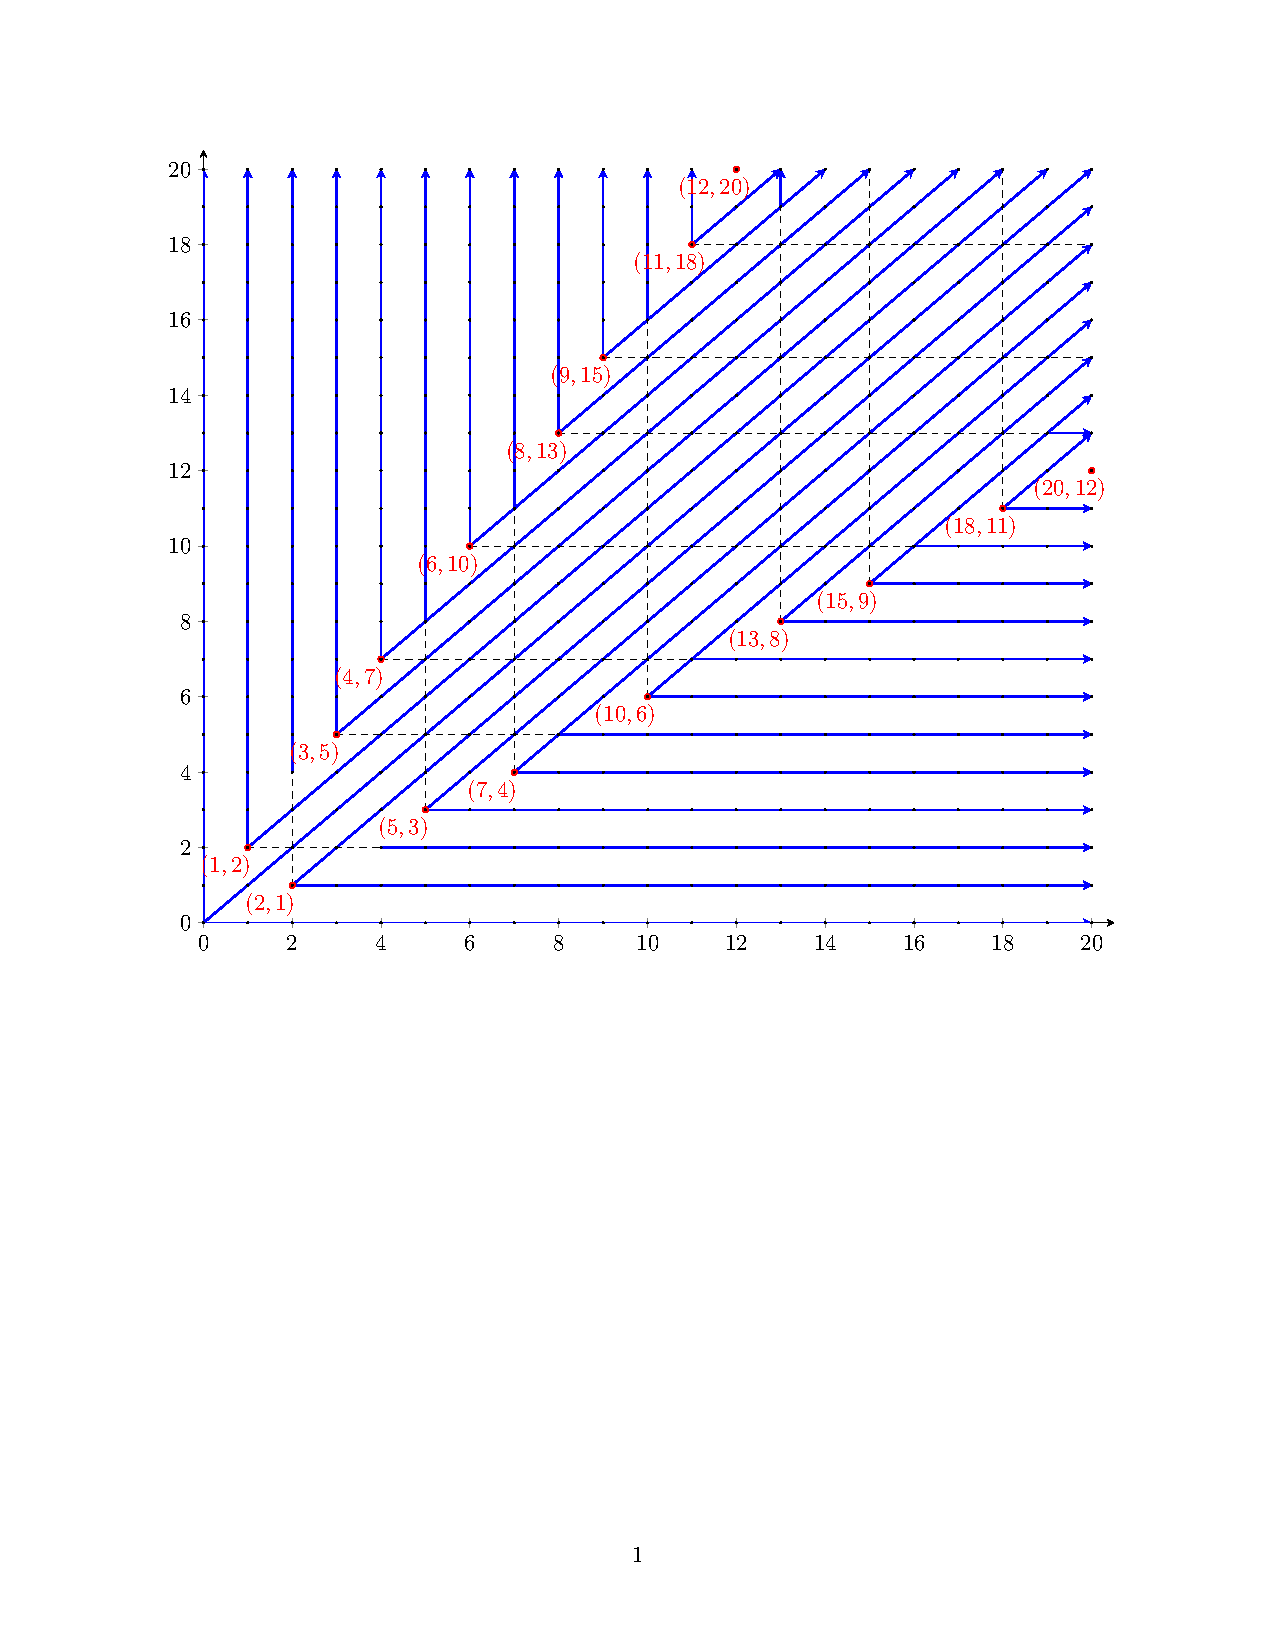
\includegraphics[scale=0.4]{Excursion_1_graphs.pdf}
	\centering
\end{frame}

\begin{frame}
	\frametitle{Basic Results}
	\pause
	\begin{proposition}{}{1}
		There are no positions that are both losing and winning. That is, $\mathcal{L} \cap \mathcal{W} =\varnothing$. Also, $(0,0)$ is a losing position.
	\end{proposition}
	\pause
	\begin{proposition}{}{2}
		Every position is either winning or losing. Also, $\mathcal{L} $ and $\mathcal{W} $ form a partition on $\mathbb{N}^2$.
	\end{proposition}
	\pause
	\begin{proposition}{}{3}
		If $(x,y)$ is a losing position, then $(y,x)$ is a losing position.
	\end{proposition}
\end{frame}

\begin{frame}
	\frametitle{The First Theorem}
	\begin{theorem}{}{1}
		Let $\lambda_n=(x,y)$ be the $n$th losing position when ordered by $\left| \lambda  \right|=x+y $, and where $(0,0)$ is the $0$th losing position. Then
		\[
			\lambda_n =(x,x+n)
		.\]
		Additionally,
		\[
			x=\min \left\{ a\in\mathbb{N} \mid \forall k<n\left( \lambda_k=(\alpha ,\beta  \right) \implies a\neq \alpha,\beta   \right\} 
		.\]
		More simply, $x$ is the smallest number that has not been ``used up'' by another losing position, and $y=x+n$.
	\end{theorem}
\end{frame}

\section{Post-Rigorous Analysis}

\begin{frame}[fragile]
	Theorem \ref{thm:1} is very important, because it lets us compute losing positions very easily with a Python script.
	\begin{lstlisting}[language=Python]
	#!/usr/bin/env python3
	avoid = set()
	losing = []
	y_int = 1
	MAX = 1000 # maximum number of tiles on board

	for x in range(1, MAX+1):
		if x not in avoid:
			losing.append((x,x + y_int))
			y_int += 1
	\end{lstlisting}\pause
	People were looking for patterns in the differences between the number of tiles, but there were no \emph{obvious} patterns. But a pattern exists, and theorem \ref{thm:1} lets us compute enough numbers to find it.
\end{frame}

\begin{frame}
	\frametitle{Differences}
\only<1>{
	\begin{center}
		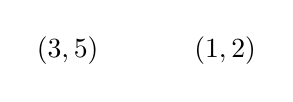
\begin{tikzpicture}
			\node at (-1,0) {$(3,5)$};
			\node at (1,0) {$(1,2)$};
		\end{tikzpicture}
	\end{center}
}
\only<2>{
	\begin{center}
		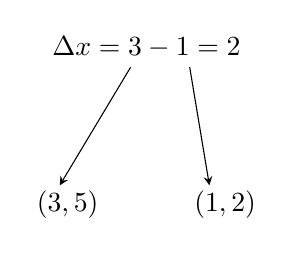
\begin{tikzpicture}
			\node (C) at (-1,0) {$(3,5)$};
			\node (B) at (1,0) {$(1,2)$};
			\node (A) at (0,2) {$\Delta x=3-1=2$};
			\draw[-stealth] (0.55,1.75) -- (0.8,0.25);
			\draw[-stealth] (-0.2,1.75) -- (-1.1,0.25);
		\end{tikzpicture}
	\end{center}
}

\end{frame}

\begin{frame}
	\frametitle{Differences}
	\begin{center}
	\begin{tabular}{|c|c|}
		\hline
		$\lambda_n$ &$\Delta x$\\
		\hline
		$(0,0)$&0\\
		$(1,2)$&1\\
		$(3,5)$&2\\
		$(4,7)$&1\\
		$(6,10)$&2\\
		$(8,13)$&2\\
		$(9,15)$&1\\
		$(11,18)$&2\\
		\hline
	\end{tabular}
	\begin{tabular}{|c|c|}
		\hline
		$\lambda_n$ &$\Delta x$\\
		\hline
		$(12,20)$&1\\
		$(14,23)$&2\\
		$(16,26)$&2\\
		$(17,28)$&1\\
		$(19,31)$&2\\
		$(21,34)$&2\\
		$(22,36)$&1\\
		$(24,39)$&2\\
		\hline
	\end{tabular}
	\begin{tabular}{|c|c|}
		\hline
		$\lambda _n$ &$\Delta x$\\
		\hline
		$(25,41)$&1\\
		$(27,44)$&2\\
		$(29,47)$&2\\
		$(30,49)$&1\\
		$(32,52)$&2\\
		$(33,54)$&1\\
		\hline
	\end{tabular}
	\end{center}
\end{frame}

\begin{frame}
	\frametitle{Differences}
	\[
		121221212212212122121
	\]
	\pause
	\begin{itemize}
		\item<2-> Only 2s and 1s
		\item<3-> Never more than one 1 in a row
		\item<4-> Never more than two 2s in a row
	\end{itemize}
\end{frame}

\begin{frame}
	\frametitle{Differences}
	\begin{center}
		\begin{tikzpicture}
			\node at (0,3) {121221212212212122121};
			\only<2>{
				\node at (0,2) {12122121};
				\draw[red] (-1.83,2.82) -- (-1.64,2.82);
				\draw[red] (-1.44,2.82) -- (-1.06,2.82);
				\draw[red] (-0.87,2.82) -- (-0.68,2.82);
				\draw[red] (-0.48,2.82) -- (-0.10,2.82);
				\draw[red] (0.48,2.82) -- (0.10,2.82);
				\draw[red] (1.83,2.82) -- (1.64,2.82);
				\draw[red] (1.44,2.82) -- (1.06,2.82);
				\draw[red] (0.87,2.82) -- (0.68,2.82);

				\draw[red,-stealth] (-1.735,2.80) -- (-0.80, 2.2);
				\draw[red,-stealth] (-1.25,2.80) -- (-0.60, 2.2);
				\draw[red,-stealth] (-0.775,2.80) -- (-0.35,2.2);
				\draw[red,-stealth] (-0.29,2.80) -- (-0.15,2.2);
				\draw[red,-stealth] (1.735,2.80) -- (0.80, 2.2);
				\draw[red,-stealth] (1.25,2.80) -- (0.60, 2.2);
				\draw[red,-stealth] (0.775,2.80) -- (0.35,2.2);
				\draw[red,-stealth] (0.29,2.80) -- (0.15,2.2);
			}
			\only<3>{
				\node at (0,2) {12122121};
				\node at (0,1) {121};
				\draw[red] (-0.58,1.82) -- (-0.39, 1.82);
				\draw[red] (-0.19,1.82) -- (0.19,1.82);
				\draw[red] (0.58,1.82) -- (0.39, 1.82);

				\draw[red,-stealth] (-0.485,1.8) -- (-0.25,1.2);
				\draw[red,-stealth] (0,1.8) -- (0,1.2);
				\draw[red,-stealth] (0.485,1.8) -- (0.25,1.2);
			}
			\only<4->{
				\node at (0,2) {12122121};
				\node at (0,1) {121};
				\node at (0,0) {1};
				\draw[red] (-0.1,0.82) -- (0.1,0.82);
				\draw[red,-stealth] (0,0.8) -- (0,0.2);
			}
		\end{tikzpicture}
	\end{center}
	\only<5>{What if we do the same thing, but in reverse?}
\end{frame}

\section{Investigation of the Sequence}
\begin{frame}
	\frametitle{Formalism}
	\begin{itemize}
		\item<1-> We need a formal definition of our sequence.
		\item<2-> ``Counting the 2s'' is very hard to formalize.
		\item<3-> We need to look for more patterns.
		\item<4-> To do this, we should compute a few of these strings.
	\end{itemize}
\end{frame}

\begin{frame}
	\frametitle{Formalism}
	\begin{center}
		\begin{tikzpicture}
			\node at (0,3) {1};
			\node at (0,2) {121};
			\node at (0,1) {12122121};
			\node at (0,0) {121221212212212122121};
			\only<2,7>{
				\draw[red] (-0.1,2.82) -- (0.1,2.82);
				\draw[red] (-0.3,2.2) -- (-0.3,1.82) -- (-0.08,1.82) -- (-0.08,2.2) -- (-0.3,2.2);
				\draw[red,-stealth] (0,2.8) -- (-0.17,2.22);
			}
			\only<3,6>{
				\draw[red] (-0.3,1.82) -- (0.3,1.82);
				\draw[red] (-0.2,1.2) -- (-0.2,0.82) -- (-0.8,0.82) -- (-0.8,1.2) -- (-0.2,1.2);
				\draw[red,-stealth] (0,1.8) -- (-0.5,1.22);
			}
			\only<4,5>{
				\draw[red] (-0.8,0.82) -- (0.8,0.82);
				\draw[red] (-0.48,-0.18) -- (-2.02,-0.18) -- (-2.02, 0.2) -- (-0.48,0.2) -- (-0.48,-0.18);
				\draw[red,-stealth] (0,0.8) -- (-1,0.22);
			}
			\only<5>{
				\draw[red] (0.48,-0.18) -- (2.02,-0.18) -- (2.02, 0.2) -- (0.48,0.2) -- (0.48,-0.18);
				\draw[red,-stealth] (0,0.8) -- (1,0.22);
			}
			\only<6>{
				\draw[red] (0.2,1.2) -- (0.2,0.82) -- (0.8,0.82) -- (0.8,1.2) -- (0.2,1.2);
				\draw[red,-stealth] (0,1.8) -- (0.5,1.22);
			}
			\only<7>{
				\draw[red] (0.3,2.2) -- (0.3,1.82) -- (0.08,1.82) -- (0.08,2.2) -- (0.3,2.2);
				\draw[red,-stealth] (0,2.8) -- (0.17,2.22);
			}
		\end{tikzpicture}
	\end{center}
\end{frame}

\begin{frame}
	\frametitle{Formalism}
	Let's call the $n$th string in this sequence $\Phi (n)$. This means
	\begin{align*}
		\Phi (1)&=1\\
		\Phi (2)&=121\\
		\Phi (3)&=12122121\\
		\Phi (4)&=121221212212212122121\\
			&\;\;\vdots
	\end{align*}
	\pause
	If our last slide is correct, we should be able to recursively define $\Phi $ as
	\[
		\Phi (n)=\Phi (n-1)\oplus \Psi  \oplus \Phi (n-1)
	,\]
	where $\Psi  $ is some unknown string.
	\pause
	
	The $\oplus $ operation is \textbf{string} \textbf{concatenation}.
\end{frame}

\begin{frame}
	\frametitle{Identifying $\Psi  $}
	\begin{center}
		\begin{tikzpicture}
			\only<1>{
				\node at (0,3) {1};
				\node at (0,2) {121};
				\node at (0,1) {12122121};
				\node at (0,0) {121221212212212122121};
			}
			\only<2->{
				\node at (0,3) {meeooowoww};
				\node at (0,2) {2};
				\node at (0,1) {22};
				\node at (0,0) {22122};
			}
			\only<3>{
				\draw[red] (-0.1,1.82) -- (0.1,1.82);
				\draw[red,-stealth] (0,1.8) -- (-0.1,1.22);
				\draw[red,-stealth] (0,1.8) -- (0.1,1.22);
				\draw[red] (-0.2,0.8) -- (-0.01,0.8);
				\draw[red] (0.2,0.8) -- (0.01,0.8);
			}
			\only<4,5>{
				\draw[red] (-0.2,0.82) -- (0.2,0.82);
				\draw[red,-stealth] (0,0.82) -- (-0.3,0.22);
				\draw[red,-stealth] (0,0.82) -- (0.3,0.22);
				\draw[red] (-0.1,-0.18) -- (-0.5,-0.18);
				\draw[red] (0.1,-0.18) -- (0.5,-0.18);
			}
			\only<5,6>{
				\draw[blue] (-0.1,-0.18) -- (0.1,-0.18) -- (0.1,0.18) -- (-0.1,0.18) -- (-0.1,-0.18);
			}
			\only<6>{
				\draw[blue,-stealth] (2,-0.18) edge [bend left=60] (0,-0.18);
				\node[blue] at (2,0) {$\Phi (1)$};
			}
		\end{tikzpicture}
	\end{center}
\end{frame}

\begin{frame}
	\frametitle{Identifying $\Psi $}
	\begin{align*}
		\Psi (1)&=2\\
		\Psi (2)&=22\only<2->{=\Psi (1)\oplus \Psi (1)}\\
		\Psi (3)&=22122\only<2->{=\Psi (2)\oplus\Phi (1)\oplus \Psi (2)}
	.\end{align*}
	\only<3>{What if we try $\Psi (n)=\Psi (n-1)\oplus \Phi (n-2)\oplus \Psi (n-1)$, where $\Phi (0)$ is the empty string and $\Psi (1)=2$?}
\end{frame}

\begin{frame}
	\frametitle{Definitions}
	\begin{definition}{Generating Functions}{1}
		Let $\Phi$ be the function satisfying
		\[
			\Phi (n)=
			\begin{cases}
				1,&n=1\\
				\Phi (n-1)\oplus \Psi (n-1)\oplus \Phi (n-1),&n>1
			\end{cases}
		.\]
		Let $\Psi$ be the function satisfying
		\[
			\Psi (n)=
			\begin{cases}
				2,&n=1\\
				\Psi (n-1)\oplus \Phi (n-2)\oplus \Psi (n-1),&n>1
			\end{cases}
		.\]
		Also let $\Phi (0)$ and $\Psi (0)$ both be the empty string.
	\end{definition}
\end{frame}

\begin{frame}
	\frametitle{Definitions}
	\begin{definition}{Differences}{2}
		Let $\lambda_n=(x_n,y_n)$ and $\lambda_{n-1}=(x_{n-1},y_{n-1})$. Then define $\Delta x_n=x_n-x_{n-1}$.
	\end{definition}
	\pause
	\begin{definition}{Losing String}{3}
		Let $\mathfrak{X}(n)$ be the string formed from the first $n$ values of $\Delta x$. That is,
		\[
			\mathfrak{X} (n)=\bigoplus_{i=1}^n \Delta x_n
		.\]
	\end{definition}
\end{frame}

\begin{frame}
	\frametitle{The Fundamental Theorem of the Tile Game}
	What we want to show is this:
	\pause
	\begin{theorem}{Fundamental Theorem}{2}
		For all $n\in\mathbb{N}$, there exists some $\omega \in\mathbb{N}$ such that $\Phi (n)=\mathfrak{X}(\omega  )$.
	\end{theorem}
	\pause
	\begin{corollary}{}{1}
		For all $\omega \in\mathbb{N}$, there exists $n\in\mathbb{N}$ such that $\mathfrak{X}(\omega )$ is a substring of $\Phi (m)$ for all $m\geq n$.
	\end{corollary}
\end{frame}

\section{Discussion}
\begin{frame}
	\frametitle{But does it work?}
	\only<1->{Before I was able to prove the theorem, I verified it worked up to positions with $400\cdot 10^{6}$ tiles in the starting position.}
	\pause

	I eventually proved the theorem with an induction argument, which isn't too difficult to understand once you know the motivation behind it, but the motivation is very messy and I don't have time to explain it or the proof in this presentation.
	\pause

	If you're interested in the proof and the various lemmas required, feel free to ask me about it.
\end{frame}

\begin{frame}
	\frametitle{$\Phi $-like Occurances}
	One interesting thing about the game is the number of places $\Phi $ or $\Phi $-like sequences appear.
\end{frame}

\begin{frame}
	\frametitle{Fibonacci Connections}
	One fascinating thing about the problem is its many connections to the Fibonacci numbers.
	\pause
	\begin{proposition}{}{4}
		Let $\left\lVert S \right\rVert $ be the length of the string $S$, and let $T(S)$ be the sum of all characters in the string $S$. Then
		\[
			\left\lVert \Phi (n) \right\rVert =F_{2n},\quad \left\lVert \Psi (n) \right\rVert =F_{2n-1}
		,\]
		\[
		T(\Phi (n))=F_{2n+1}-1,\quad T(\Psi (n))=F_{2n}+1
		.\]
	\end{proposition}
\end{frame}
\begin{frame}
	\frametitle{Fibonacci Connections}
	\begin{proposition}{}{5}
		For all $n\in\mathbb{Z}^+$,
		\[
			\left( F_{2n},F_{2n+1} \right) \in \mathcal{L} 
		,\]
		\[
			\left( F_{2n+1}-1,F_{2n+2}-1 \right) \in \mathcal{L} 
		.\]
	\end{proposition}
	\pause
	\begin{proposition}{}{6}
		Let $(a,b)\in \mathcal{L} $. Then $(a+b,a+2b)\in \mathcal{L} $.
	\end{proposition}
\end{frame}
\begin{frame}
	\frametitle{Fibonacci Connections}
	\begin{proposition}{}{7}
		Let
		\[
			\mathcal{F} =\left\{ \left( F_{2n},F_{2n+1} \right)  \mid n\in\mathbb{Z}^+ \right\} \subset \mathcal{L} 
		.\]
		Then every losing position $\lambda \in \mathcal{L} $ can be written as
		\[
			\lambda =\sum_{n=1}^{N} c_n\left( F_{2n},F_{2n+1} \right) 
		\]
		for some $\left\{ c_{n} \right\}_{n=1}^N\subset \mathbb{N}$. 
	\end{proposition}
	\pause
	One remark about proposition \ref{prp:7} is that not all linear combinations of $\mathcal{F} $ are losing positions, but all losing positions are linear combinations of $\mathcal{F} $.
\end{frame}
\begin{frame}
	\frametitle{Fibonacci Connections}
	\begin{corollary}{}{2}
		Corollary of proposition \ref{prp:7}. Let $(x,y)\in \mathcal{L} $. Then there exists $\left\{ c_n \right\}_{n=1}^N\subset \mathbb{N}$ such that
		\[
			x+y=\sum_{n=1}^{N} c_n\left( F_{2(n+1)} \right) 
		.\]
	\end{corollary}
	\pause
	\begin{corollary}{}{3}
		For all $(x,y) \in \mathcal{L} $ such that $x+y < F_{2n}+F_{2n+1} $, then
		\[
			(x,y)+\left( F_{2n},F_{2n+1} \right) \in \mathcal{L} 
		.\]
	\end{corollary}
\end{frame}
\end{document}
